\documentclass{article}
\pagestyle{empty}
\usepackage{amsmath,amssymb}
\usepackage{xcolor}
\usepackage{tikz}
\usetikzlibrary{arrows.meta,positioning,calc}

\newsavebox{\figbox}
\newcommand{\fs}{\fontsize{6}{7}\selectfont}

\newcommand{\sqmark}[3]{\fill[#1] ([shift={(-1.3pt,-1.3pt)}]#2,#3) rectangle ([shift={(1.3pt,1.3pt)}]#2,#3);}
\newcommand{\trimark}[3]{\fill[#1] ([shift={(0pt,1.8pt)}]#2,#3) -- ([shift={(-1.6pt,-1.1pt)}]#2,#3) -- ([shift={(1.6pt,-1.1pt)}]#2,#3) -- cycle;}

\begin{document}
\savebox{\figbox}{%
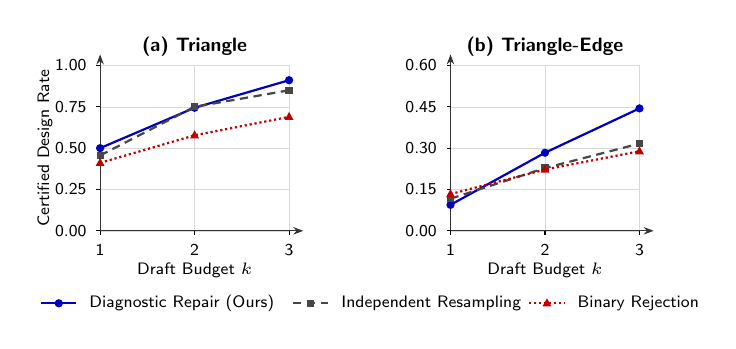
\begin{tikzpicture}[font=\sffamily\scriptsize]
% Padding box
\path (-0.92, -1.10) rectangle (7.70, 2.55);

% Y-axis label
\node[rotate=90, font=\sffamily\fs, anchor=center] at (-0.70, 1.05) {Certified Design Rate};

% Panel (a): Triangle (y in [0, 1.0] mapped to [0, 2.1])
\begin{scope}[xshift=0cm]
\node[font=\sffamily\scriptsize\bfseries] at (1.20, 2.34) {(a) Triangle};
\draw[gray!30, very thin] (0,0) grid[xstep=1.20, ystep=0.525] (2.40, 2.10);
\draw[-{Stealth[scale=0.75]}, black!80] (0,0) -- (2.58,0);
\draw[-{Stealth[scale=0.75]}, black!80] (0,0) -- (0,2.24);
\node[font=\sffamily\fs] at (1.20, -0.50) {Draft Budget $k$};
\foreach \x/\lbl in {0/1, 1.20/2, 2.40/3} \draw (\x,0) -- (\x,-0.05) node[below, font=\sffamily\fs]{\lbl};
\foreach \y/\lbl in {0.0/0.00, 0.525/0.25, 1.05/0.50, 1.575/0.75, 2.10/1.00} \draw (0,\y) -- (-0.05,\y) node[left, font=\sffamily\fs]{\lbl};

% Diagnostic Repair: (0.5000, 0.7444, 0.9111) * 2.1 = (1.050, 1.563, 1.913)
\draw[blue!75!black, thick] (0,1.050) -- (1.20,1.563) -- (2.40,1.913);
\foreach \x/\y in {0/1.050, 1.20/1.563, 2.40/1.913} \fill[blue!75!black] (\x,\y) circle (1.5pt);

% Independent Resampling: (0.4556, 0.7500, 0.8500) * 2.1 = (0.957, 1.575, 1.785)
\draw[black!72, thick, densely dashed] (0,0.957) -- (1.20,1.575) -- (2.40,1.785);
\foreach \x/\y in {0/0.957, 1.20/1.575, 2.40/1.785} \sqmark{black!72}{\x}{\y};

% Binary Rejection: (0.4111, 0.5778, 0.6889) * 2.1 = (0.863, 1.213, 1.447)
\draw[red!75!black, thick, densely dotted] (0,0.863) -- (1.20,1.213) -- (2.40,1.447);
\foreach \x/\y in {0/0.863, 1.20/1.213, 2.40/1.447} \trimark{red!75!black}{\x}{\y};
\end{scope}

% Panel (b): Triangle-Edge (y in [0, 0.60] mapped to [0, 2.1], factor = 3.5)
\begin{scope}[xshift=4.45cm]
\node[font=\sffamily\scriptsize\bfseries] at (1.20, 2.34) {(b) Triangle-Edge};
\draw[gray!30, very thin] (0,0) grid[xstep=1.20, ystep=0.525] (2.40, 2.10);
\draw[-{Stealth[scale=0.75]}, black!80] (0,0) -- (2.58,0);
\draw[-{Stealth[scale=0.75]}, black!80] (0,0) -- (0,2.24);
\node[font=\sffamily\fs] at (1.20, -0.50) {Draft Budget $k$};
\foreach \x/\lbl in {0/1, 1.20/2, 2.40/3} \draw (\x,0) -- (\x,-0.05) node[below, font=\sffamily\fs]{\lbl};
\foreach \y/\lbl in {0.0/0.00, 0.525/0.15, 1.05/0.30, 1.575/0.45, 2.10/0.60} \draw (0,\y) -- (-0.05,\y) node[left, font=\sffamily\fs]{\lbl};

% Diagnostic Repair: (0.0944, 0.2833, 0.4444) * 3.5 = (0.330, 0.992, 1.555)
\draw[blue!75!black, thick] (0,0.330) -- (1.20,0.992) -- (2.40,1.555);
\foreach \x/\y in {0/0.330, 1.20/0.992, 2.40/1.555} \fill[blue!75!black] (\x,\y) circle (1.5pt);

% Independent Resampling: (0.1167, 0.2278, 0.3167) * 3.5 = (0.408, 0.797, 1.108)
\draw[black!72, thick, densely dashed] (0,0.408) -- (1.20,0.797) -- (2.40,1.108);
\foreach \x/\y in {0/0.408, 1.20/0.797, 2.40/1.108} \sqmark{black!72}{\x}{\y};

% Binary Rejection: (0.1333, 0.2222, 0.2889) * 3.5 = (0.467, 0.778, 1.011)
\draw[red!75!black, thick, densely dotted] (0,0.467) -- (1.20,0.778) -- (2.40,1.011);
\foreach \x/\y in {0/0.467, 1.20/0.778, 2.40/1.011} \trimark{red!75!black}{\x}{\y};
\end{scope}

% Centered clean legend at bottom
\begin{scope}[yshift=-0.92cm]
\draw[blue!75!black, thick] (-0.75,0) -- (-0.30,0);
\fill[blue!75!black] (-0.525,0) circle (1.5pt);
\node[right, font=\sffamily\fs] at (-0.26,0) {Diagnostic Repair (Ours)};

\draw[black!72, thick, densely dashed] (2.45,0) -- (2.90,0);
\sqmark{black!72}{2.675}{0};
\node[right, font=\sffamily\fs] at (2.94,0) {Independent Resampling};

\draw[red!75!black, thick, densely dotted] (5.45,0) -- (5.90,0);
\trimark{red!75!black}{5.675}{0};
\node[right, font=\sffamily\fs] at (5.94,0) {Binary Rejection};
\end{scope}
\end{tikzpicture}%
}%
\pdfpagewidth=\wd\figbox
\pdfpageheight=\dimexpr\ht\figbox+\dp\figbox\relax
\hoffset=-1in
\voffset=-1in
\topmargin=0pt \headheight=0pt \headsep=0pt \oddsidemargin=0pt \evensidemargin=0pt
\parindent=0pt
\vbox to \pdfpageheight{\hbox to \pdfpagewidth{\usebox{\figbox}}\vss}
\end{document}
